\chapter{Anomaly Detection}


\section{Gaussian Distribution}
\begin{itemize}
    \item Say $x \in \mathbb{R}$. If $x$ is a distributed Gaussian with mean $\mu$, variance $\sigma^2$ 
    (where $\sigma$ called ``standard deviation'')

    \begin{equation}
        P(x;\mu,\sigma^2) = \frac{1}{\sqrt{2\pi}\sigma}\exp\left({-\frac{(x-\mu)^2}{2\sigma^2}}\right)
    \end{equation}
    
    \begin{figure}[!htbp]
        \centering
        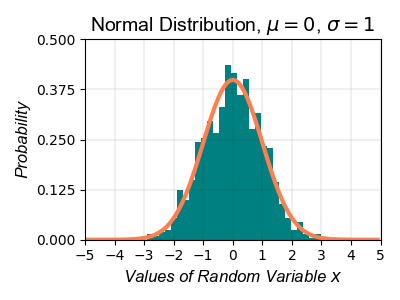
\includegraphics[width=3.2in]{./images/gaussianDistribution.png}
        \caption{Gaussian distribution}
    \end{figure}

    \item Algorithm
    \begin{enumerate}
        \item Choose features $x_i$ that you think might be indicative of anomalous examples, 
        such as ``memory use'', ``CPU load'' for monitoring computers
        
        \item Fit parameters for $\mu_1,\dots,\mu_n$ and $\sigma_1^2,\dots,\sigma_n^2$
        
        \begin{equation}
            \begin{aligned}
                \mu_j      &= \frac{1}{m} \sum_{i=1}^{m}{x^{(i)}_j}\\
                \sigma_j^2 &= \frac{1}{m} \sum_{i=1}^{m}\left(x^{(i)_j} - \mu_j\right)^2
            \end{aligned}
        \end{equation}
        
        \item Compute the probability density function 
        \begin{equation}
            P(x) = \prod_{j=1}^{n} P(x_j;\mu_j,\sigma_j^2) = \prod_{j=1}^{n} \frac{1}{\sqrt{2\pi}\sigma_j}\exp\left({-\frac{(x_j-\mu_j)^2}{2\sigma_j^2}}\right)
        \end{equation}
        
        \item Predict
        \begin{equation}
            y = \left\{
            \begin{array}{llll}
                1 & \text{if} & p(x) <    \varepsilon & \text{(anomaly)}  \\
                0 & \text{if} & p(x) \geq \varepsilon & \text{(nomal)} 
            \end{array}\right.
        \end{equation}
        
        Parameter $\varepsilon$ can be choose by observation from cross validation set.
        There are other ways, such as \emph{error metrices}, \emph{precision/recall} or, \emph{F1 score}.
    \end{enumerate}
    
    \begin{figure}[!htbp]
        \centering
        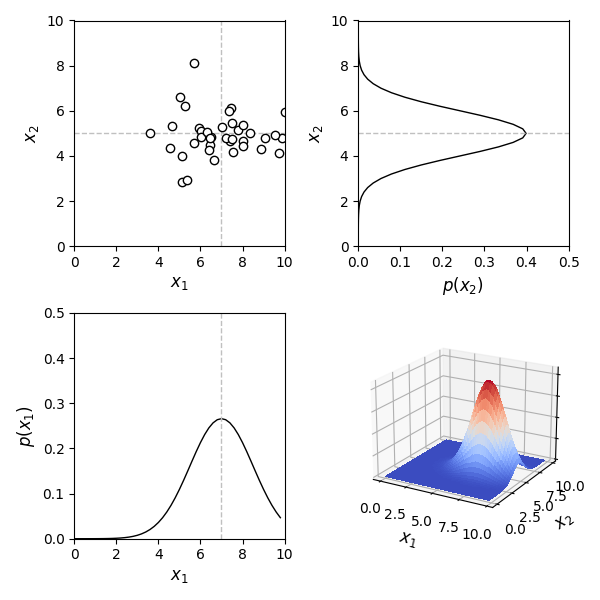
\includegraphics[width=4.2in]{./images/gaussianDistribution_3D.png}
        \caption{Gaussian distribution}
    \end{figure}

\end{itemize}


\section{Multivariate Gaussian Distribution}
\begin{itemize}
    \item The multivariate normal distribution is often used to describe any set of \emph{correlated} random variables.
    If using single-variable distribution to describe a variable-correlated dataset, 
    anomalies could be hard to excluded.
    \begin{figure}[!htbp]
        \centering
        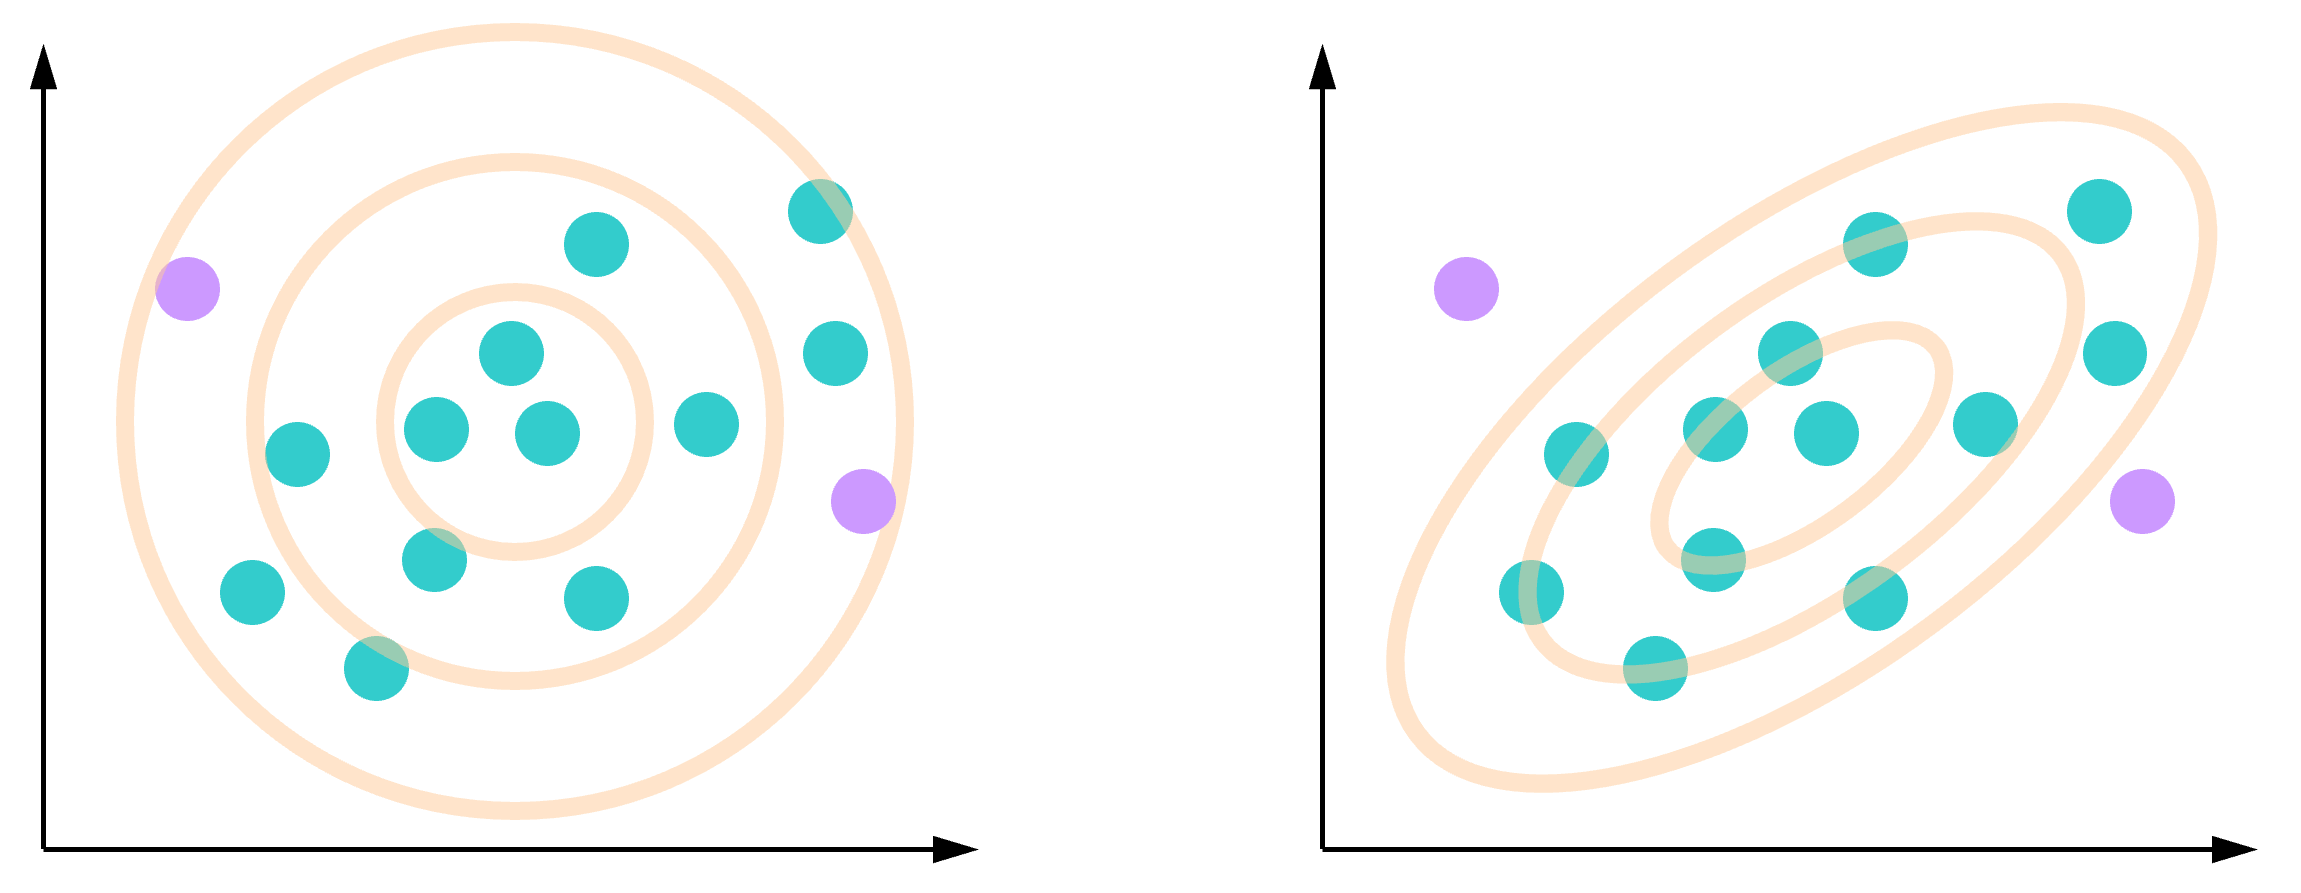
\includegraphics[width=3.6in]{./images/twoDistributionModel.png}
        \caption{Gaussian distribution with single-variate and multivariate}
    \end{figure}
    
    \item Algorithm
    \begin{enumerate}
        \item Fit model $p(x)$ by setting mean vector $\mu\in\mathbb{R}^n$ and covariance matrix $\Sigma\in\mathbb{R}^{n\times n}$
        \begin{equation}
            \begin{aligned}
                \mu    &= \frac{1}{m}\sum_{i=1}^{m} x^{(i)} \\
                \Sigma &= \frac{1}{m}\sum_{i=1}^{m} \left(x^{(i)} - \mu\right) \left(x^{(i)} - \mu\right)^T \\
            \end{aligned}
        \end{equation}

        \item Given a new example $x$, compute probability density function
        \begin{equation}
            p(x; \mu, \Sigma) = \frac{1}{ \left(2\pi\right)^{ \frac{n}{2} } \left|{\Sigma}\right|^{\frac{1}{2}}} \exp{\left(-\frac{1}{2}\left(x-\mu\right)^T\Sigma^{-1}\left(x-\mu\right)\right)}
        \end{equation}

        \item Flag an anomaly if $p(x)<\varepsilon$
    \end{enumerate}

    \item Examples.
    \begin{equation}
        \begin{array}{llll}
        \mu_1 = &\left[\begin{array}{c} 0 \\ 0 \end{array}\right] & \Sigma_1 &= \left[\begin{array}{cc} 1.0 &  0.0 \\  0.0 & 1.0 \end{array}\right] \\
        \mu_2 = &\left[\begin{array}{c} 0 \\ 0 \end{array}\right] & \Sigma_2 &= \left[\begin{array}{cc} 1.0 &  0.5 \\  0.5 & 1.0 \end{array}\right] \\
        \mu_3 = &\left[\begin{array}{c} 0 \\ 0 \end{array}\right] & \Sigma_3 &= \left[\begin{array}{cc} 1.0 & -0.5 \\ -0.5 & 1.0 \end{array}\right]
        \end{array}
    \end{equation}
    \begin{figure}[!htbp]
        \centering
        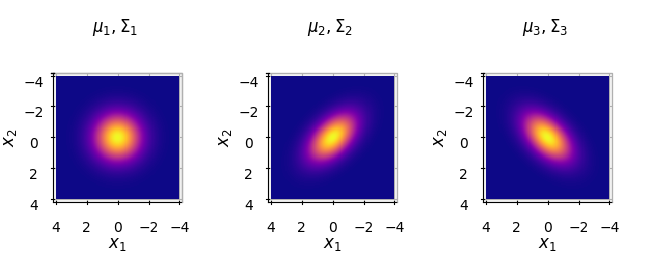
\includegraphics[width=6.2in]{./images/gaussianDistributionMultivariate.png}
        \caption{Gaussian distribution with multivariate}
    \end{figure}

\end{itemize}

    
\section{Non Gaussian Features}
\begin{itemize}
    \item Given the data set that looks like a \emph{log-normal} distribution, 
    take a log transformation of the data, then the histogram looks much more Gaussian.
    
    \item Probability density function for log-normal distribution
    \begin{equation}
        f_X(x) = \frac{1}{x\sigma\sqrt{2\pi}}\exp{\left(-\frac{\left(\ln x - \mu\right)^2}{2\sigma^2}\right)}
    \end{equation}
    
    \item Cumulative distribution function for log-normal distribution
    \begin{equation}
        F_X(x) = \frac{1}{2} \left[1 + \text{erf}\left(\frac{\ln x - \mu}{\sigma \sqrt{2}}\right) \right]
    \end{equation}
    
    \begin{figure}[!htbp]
        \centering
        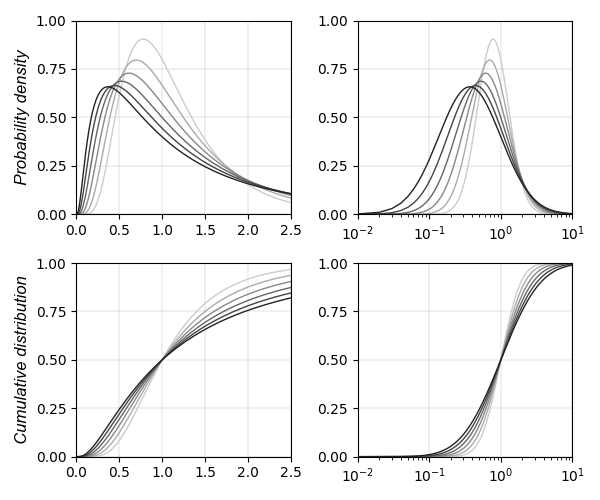
\includegraphics[width=4.2in]{./images/logNormalDistribution.png}
        \caption{Log-normal distribution}
    \end{figure}
    
\end{itemize}

